\section{Research Methodology}
\label{sec:1_introduction_methodology}
The research field of this thesis is moving fast due to technological advances and the continuous generation of new contributions in ML. Consequently, an iterative research methodology was followed. The main idea of this cyclical process is that the knowledge acquired in its initial phase helps to design an increasingly promising technique,
either in terms of accurate results, or in terms of concept, offering originality and remarkable contributions. Fig. \ref{ch1:research-emthodo} shows the different phases of this research methodology.
These phases are briefly described below:

\begin{figure}[!ht]
    \centering
    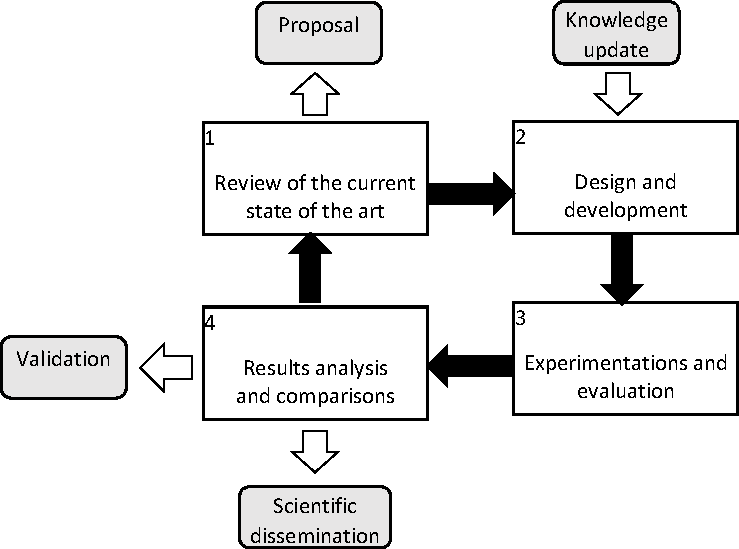
\includegraphics[width=.8\textwidth]{1_introduction/figures/fig_research-methodo.pdf}
    \caption{The research methodology of the thesis.}
    \label{ch1:research-emthodo}
\end{figure}

\begin{enumerate}
    \item \textbf{Review of the current state-of-the-art:}  The main objective of this phase is to investigate the state of the art related to the field under consideration to identify problems and/or challenges. To achieve this, the related bibliography is used, reviewing publications from the scientific community published in journals, and proceedings of international congresses. The knowledge acquired in this phase should lead to a proposal to address the identified challenges.

 \item \textbf{Design and development:} In this phase, a novel proposal to solve the identified challenges is designed and developed. To this end, previously acquired or updated knowledge is used to ensure that the solution is always up-to-date with the current state of the art.

\item \textbf{Experimentation and evaluation:} The goal of this phase is to test the proposals resulting from the previous step to a process of experimentation. To carry out this procedure, it is crucial to provide some criteria and evaluation methods with which the results will be compared in the subsequent phase. All these criteria and methods must be built using the knowledge acquired in the first stage of the methodology.

\item \textbf{Results analysis and comparison:} After carrying out experimentation, results must be analyzed and compared with those obtained in the state-of-the-art. At this point, it is needed to check if the results obtained are enough to address the challenges identified in the first phase. In such a case, another methodological cycle begins to approach the following challenge identified or to keep working with the challenge under consideration if it was not still solved. In this stage, conclusions must be drawn from analyses of results, and knowledge obtained must be materialized in scientific dissemination, either
through journals, or conferences.

\end{enumerate}